\documentclass[12pt]{article}
\usepackage[english]{babel}
\usepackage[utf8x]{inputenc}
\usepackage{amsmath}
\usepackage{tablefootnote}
\usepackage{amssymb}
\usepackage{graphicx}
\usepackage{float}
\usepackage[colorinlistoftodos]{todonotes}
\usepackage{geometry}
\usepackage{booktabs}
\usepackage{siunitx}
\usepackage{tabularx}
\usepackage{placeins}

\usepackage[style=authoryear,backend=biber,hyperref=true,citestyle=authoryear-comp]{biblatex}
\usepackage[colorlinks=true,linkcolor=blue,citecolor=blue,urlcolor=blue]{hyperref}
\hypersetup{
    colorlinks=true,
    linkcolor=blue,
    citecolor=blue,
    urlcolor=blue
}
\addbibresource{references.bib}
\geometry{letterpaper, margin = 2 cm}
\usepackage{subcaption}

\begin{document}



\newcommand{\HRule}{\rule{\linewidth}{0.5mm}} 

\thispagestyle{empty}

\begin{center}


\includegraphics[width=0.45\textwidth]{amse_logo.png}\\
\vspace{0.5cm}
\textsc{\huge Aix Marseille School of Economics} \\[0.3cm]

\vspace{2cm}


\textsc{\LARGE Final Evaluation in the courses of}\\[0.4cm]
\textsc{\large Predictive Methods}\\[0.1cm]
\textsc{\large Machine \& Statistical Learning,} \\[0.1cm]
\textsc{\large Information Reduction Methods}


\vspace{1cm}


\HRule \\[0.4cm]
{ \huge \textbf{Car Price Prediction} \\[0.5cm] 
Development of a mixed machine learning model to predict car prices
}\\[0.4cm]
\HRule \\[3cm]


\begin{minipage}[t]{0.8\textwidth}
	\begin{itemize}
    \item[\emph{Authors:}] Honorine DESILLES, \\
    Olivier JAYLET, \\
    Marcel PENDA 
    \item[\emph{Program:}] M.Sc. Econometrics, Big Data and statistics
	\item[\emph{Professors:}] Pierre MICHEL, \\ Sullivan HUE
	\item[\emph{Submission:}] \today
	\end{itemize}
\end{minipage}




\end{center}
\newpage

\renewcommand{\contentsname}{Table of contents}\tableofcontents

\newpage

\section{Introduction}
Current economic, social and environmental challenges raise many questions regarding the future of transportation. Particularly in industrialized countries, trends and new concepts such as sharing economy, circular economy or the general transition towards decarbonisation drive societal thoughts and behaviour. In many countries individual transportation, and thus the automotive industry continue to constitute a crucial economic pillar (\cite{huang2023dvmcar}). However, while European car exports to China and the USA are still increasing, the sales volume for \textit{second hand} cars is much larger in most countries. Generating twice the volume than the new automobile market, the second hand car market represents the largest retail sector in the US economy (\cite{Celik2019}). \\

\noindent Due to these trends and challenges, fast and accurate car price assessments are crucial for both, sellers and buyers. Fluctuations in car preferences, and thus supply and demand make it important to make fast sales and calculate the ideal price. Online marketplaces such as AutoScout, leboncoin or ebay aim to facilitate the process of matching sellers and buyers of used cars. Another case is the evaluation of leasing cars after the contract period and the optional acquisition (\cite{su142417034}). So far, however, only few researchers addressed this question using sophisticated machine learning methods and large data. One reason for this might be that accurately estimating car prices depends on various factors and characteristics. This makes it often difficult for laypersons but also professionals to adequately value and exchange cars at the right price. This might be even more challenging when viewing and assessing the car online and/or only based on few information \cite{Bilen2021}. Even though researchers like \cite{Pudaruth2014} show that some factors such as a car's age, model, mileage or horsepower already may explain it's price to some extent, predicting an accurate resale value remains a difficult task. Thus, data driven price evaluation based on more complex machine learning algorithms may be a fast, efficient and convenient method for the task at hand.\\

\noindent The existing literature on price prediction for used cars shows different empirical approaches. For instance, \cite{Pudaruth2014} compared a multiple linear regression, k-nearest neighbours, and decision tree models using car data from Mauritius. According to him, more sophisticated methods such as neural networks or concatenated models might be a good approach to increase the accuracy of car price predictions. Similarly, \cite{chen2017comparative} trained a linear regression and random forest model on a dataset of 100,000 used cars in China. Their findings suggest to apply more complex models with a large number of variables to find a better model fit. This is in line with \cite{Samruddhi2020} who present another KNN model with a prediction accuracy of 85\% but also propose advanced machine learning methods for better car price predictions. That said, \cite{Karakoç2020} fitted artificial neural networks based on a small data set of 1000 observation, obtaining a model accuracy of 91\% but arguing that a larger database would improve their results. Among their tree based models, \cite{Gajera2021} find the random forest and XGBoost to provide the best predictions with accuracy rates of 93\% and 92\% respectively. \footnote{Regarding the error metric, the researchers obtain a root mean squared error (RMSE) of 3,702.34 and 3,980.77 respectively.} Comparing a support vector machine (SVM) and ANN model, \cite{Bilen2021} finds that the ANN surpasses the SVM with a model accuracy of 89\%. A different approach was chosen by \cite{yang2018ai} who trained convolutional neural networks (CNNs) on a rather samll sample of 1,400 car images to predict the corresponding price. Their best test set results show an accuracy of 98\%. \footnote{In terms of RMSE, their best model achieves a score of 10,577.47} Besides applying their model to help in product design, they propose to extend its application to used car sales where prices must be evaluated quickly but are difficult to determine. In 2021, due to the mentioned sparse data problem, \cite{huang2023dvmcar} created a new large-scale automotive dataset including image data for visual applications. This database constitutes the main database for this elaboration and will be further presented in the next section. \\

\noindent Given the above mentioned findings and following the repeatedly mentioned recommendations for further research to fit \textit{more complex} models on \textit{larger data}, this elaboration aims at estimating and comparing some of the most promising algorithms using the extensive DVM-Car data set provided by \cite{huang2023dvmcar}. To do so, we will first present the descriptive statistics as well as the preprocessing of our data. In a next step, we will briefly introduce, apply and fine tune the hyperparameters of different machine learning algorithms. More precisely, our empirical analysis will present and compare the results of an XGBoost, KNN and ANN model fitted on categorical and numerical data as well as the results of an image based model. In a last step, following the suggestions of \cite{Pudaruth2014}, we propose a concatenated machine learning model exploiting all data available, i.e. categorical, numerical an visual data to improve our overall model performance.\\

\noindent What you found (highlight of your key results: \\
\noindent To be written in the end when all the models were interpret!



\section{Materials and Methods}
\subsection{Database}
\noindent La base de données sur laquelle nous avons travaillé tout au long de ce projet, a été créé par des chercheurs Jingmin Huang et Bowei Chen. Leur but premier était de permettre l'étude du design des voitures. Nous l'avons cependant utilisé afin de prédire et comprendre les prix des voitures. 

\noindent Ces données étant nombreuses et complexes, notre travail de preprocessing nous aura prit beaucoup de temps. Voici comment se structurent les tables. 

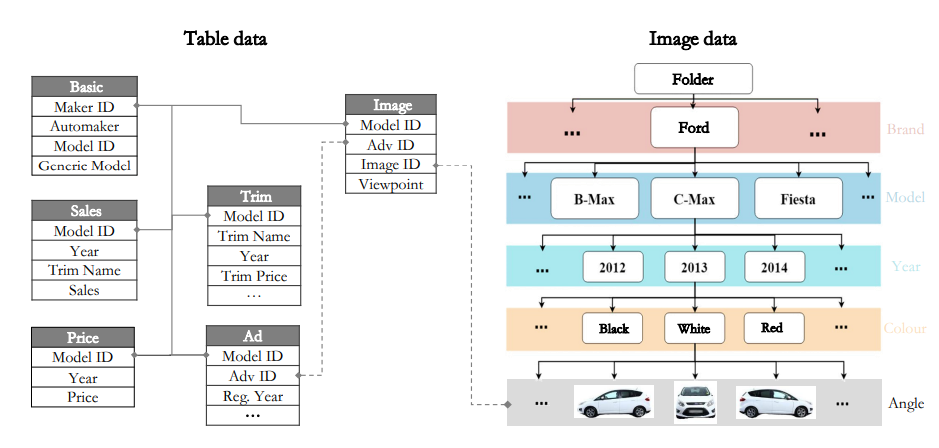
\includegraphics[width=0.9\textwidth]{general_data_tables.png}\\
\vspace{0.5cm}

\noindent La base de données contient cinq fichiers CSV, dont une qui permet de créer des liens pour lier les données tabulaires aux images. Les données en image sont stockées dans un fichier ZIP, dans lequel, un chemin d'accès doit être retracé pour accéder à l'image d'une voiture en particulier.

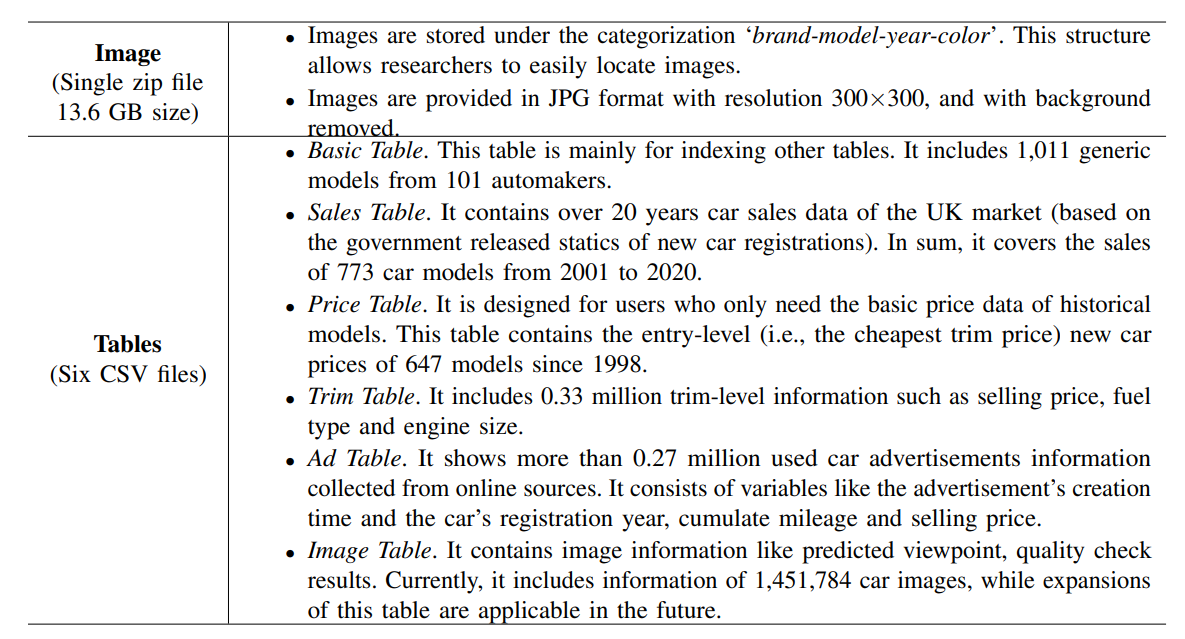
\includegraphics[width=0.9\textwidth]{overviewDVMdata.png}\\
\vspace{0.5cm}

\noindent Nous avons décidé d'utiliser les tables \textit{Trim} et \textit{Ad} pour les données numériques et catégoriques.
\noindent Tandis que pour les images, nous avons retracé les chemins d'accès grace aux tables \textit{Price} et \textit{Image}. 

\subsubsection{Categorical and numerical data}

\paragraph{Data Description}
~~\\
\\

\noindent In order to create a dataset comprising numerical and categorical data, we have decided to merge two databases made available to us, as indicated in the 'voir papier'.\\

\noindent The first table is named Ad table. It is a dataset that includes 268,255 observations and 24 variables. These variables describe the characteristics of vehicles such as size, color, price, model, etc. These data can be categorical, such as the car manufacturer, model, or gearbox type. There are also numerical data such as engine power and price. Many missing data are present in this table, notably in the columns colors, annual tax, average mpg, or top speed. We will explain in the next section, named preprocessing, how we handled these missing data. Additionally, outliers have been identified in this table, which may be due to poorly entered data or the presence of unique car models very different from others. These anomalies will be thoroughly examined in the preprocessing of the data.\\

\noindent The second table is named Trim.csv. This table consists of 335,562 observations and 9 variables. We only have the variable indicating the gas emissions of the cars.\\

\noindent Following the merging of these two tables, we obtained a final table of 213K observations before preprocessing. The objective of our work is to predict the price of cars, and our dependent variable will be the 'price' variable.\\

\noindent Here is the dictionary of variables that we have selected for our final dataset.\\



\begin{table}[ht]
    \centering
    \caption{Dictionary of Variables}
    \label{tab:variables}
    \begin{tabularx}{\textwidth}{lclX}
        \toprule
        \textbf{Variable} & \textbf{Type} & \textbf{Description} \\
        \midrule
        Price & Float & Vehicle price. \\
        Runned\_Miles & Float & Miles traveled by the vehicle. \\
        Engin\_size & Float & Vehicle engine size. \\
        Engine\_power & Float & Vehicle engine power. \\
        Wheelbase & Float & Vehicle wheelbase. \\
        Height & Float & Vehicle height. \\
        Width & Float & Vehicle width. \\
        Length & Float & Vehicle length. \\
        Average\_mpg & Float & Average fuel consumption in miles per gallon. \\
        Gas\_emission & Float & Vehicle gas emission. \\
        Top\_speed & Float & Vehicle maximum speed. \\
        Seat\_num & Int & Number of seats in the vehicle. \\
        Door\_num & Int & Number of doors of the vehicle. \\
        Body\_type & String & Vehicle type. \\
        Gear\_box & String & Gearbox type. \\
        Fuel\_type & String & Fuel type. \\
        \bottomrule
    \end{tabularx}
\end{table}

\paragraph{Descriptive Statistics}
~~\\

\noindent Descriptive statistics give us a better overview of our database.\\

\noindent First, let's look at the numerical variables. The following frequency table shows the main descriptive stats for these variables, with the number of values, mean, standard deviation, minimum, maximum and quartiles. This gives us an idea of the distribution of these variables.\\


\begin{table}[h]
    \centering
    \caption{ Descriptive statistics}
    \begin{tabular}{lrrrrrrr}
    \toprule
           & Price & Runned\_Miles & Engin\_size & Engine\_power & Height & Width & Length \\
    \midrule
     count & 200676 & 200676 & 200676 & 200676 & 200676 & 200676 & 200676 \\
     mean & 10589.9 & 52352.4 & 1.8085 & 137.959 & 1535.76 & 1885.63 & 4334.15 \\
     std & 9496.06 & 39580.4 & 0.600646 & 60.2528 & 116.157 & 149.073 & 402.895 \\
     min & 100 & 2 & 0.66 & 50 & 1112 & 1475 & 2727 \\
     25\% & 3995 & 18250 & 1.4 & 99 & 1460 & 1770 & 4052 \\
     50\% & 7950 & 46000 & 1.6 & 120 & 1495 & 1875 & 4344 \\
     75\% & 13799 & 80000 & 2 & 168 & 1615 & 2013 & 4644 \\
     max & 56750 & 222000 & 4.6 & 429 & 1951 & 2365 & 5970 \\
    \bottomrule
    \end{tabular}
\end{table}

\begin{table}[h]
    \centering
    \begin{tabular}{lrrrrrrr}
    \toprule
           & Average\_mpg & Top\_speed & Gas\_emission & Wheelbase & Seat\_num & Door\_num \\
    \midrule
     count & 200676 & 200676 & 200676 & 200676 & 200676 & 200676 \\
     mean & 51.9473 & 120.585 & 152.543 & 2636.89 & 4.92767 & 4.45066 \\
     std & 12.3794 & 15.6977 & 37.9909 & 169.992 & 0.790823 & 0.931608 \\
     min & 9.8 & 80 & 0 & 1445 & 1 & 2 \\
     25\% & 43.5 & 109 & 129.096 & 2511 & 5 & 4 \\
     50\% & 51.4 & 118 & 142.786 & 2634 & 5 & 5 \\
     75\% & 61.1608 & 130 & 167.316 & 2741 & 5 & 5 \\
     max & 134.5 & 189 & 440 & 4065 & 9 & 5 \\
    \bottomrule
    \end{tabular}
\end{table}

\FloatBarrier

\noindent Interpretation: On average, a car costs €10,589.90. (in italics) \\

\noindent The following graph (Figure 1) illustrates the distribution of our target variable, price. This boxplot reveals a tight distribution, indicating that most data are concentrated between €5,000 and €10,000, with little dispersion. The median, represented by the central line of the box, lies at €9,000, meaning that 50 % of the data are below this value.
\noindent The whiskers on the graph, generally associated with extreme values, show points on the right-hand side after the right-hand whiskers, identified as outliers. Despite efforts to clean up the price variable, reducing the range of values from €100,000 to €56,000, the graph shows the persistence of numerous outliers. By choice, we have decided to retain these values, considered less aberrant than those in our initial dataset.
\noindent This box plot shows an asymmetry in the distribution of our dependent variable.

\FloatBarrier
\begin{figure}[ht]
    \centering
    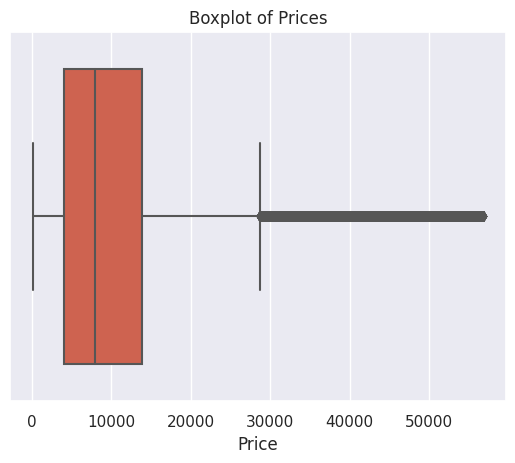
\includegraphics[width=0.45\textwidth]{boxplot price.png}
    \caption{Boxplot of prices}
    \label{fig:boxplot}
\end{figure}
\FloatBarrier

\noindent Next, we decided to show the relationship between each float variable and the price. This graphical representation proved useful for detecting outliers in the first instance, which we removed in the pre-processing step explained above. It can also be interesting to study the distribution of prices for each variable, in order to familiarize ourselves with the dataset we will later use to train our models. Finally, this approach allows us to identify trends between the independent variables and the dependent variable, price. For example, we can observe a positive correlation between vehicle price and engine power.

\begin{figure}[ht]
    \centering
    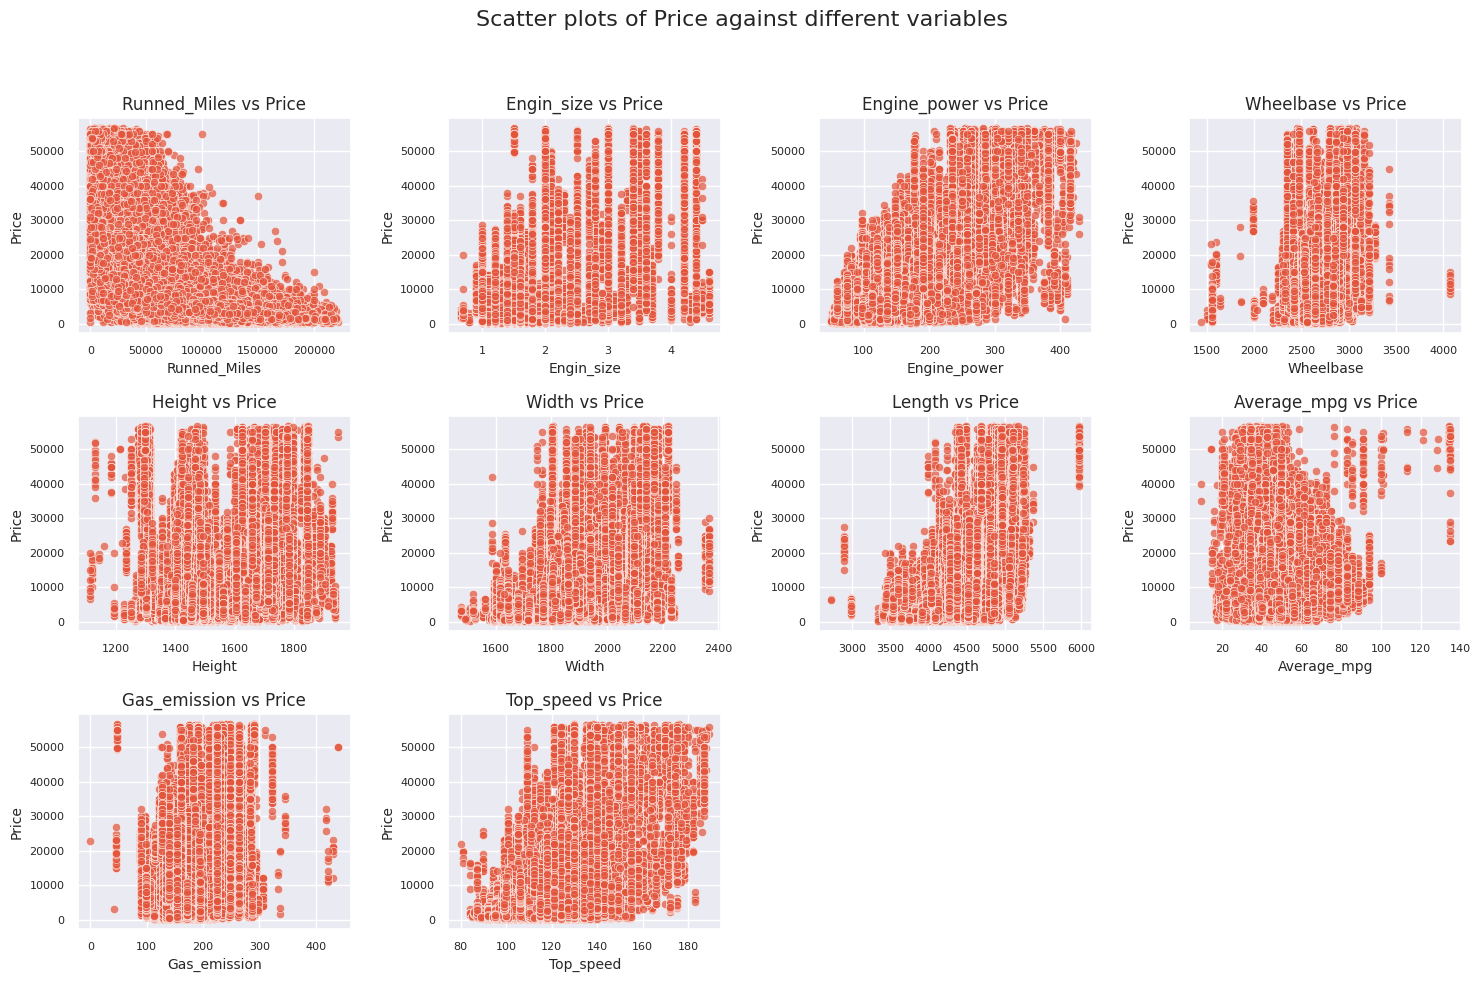
\includegraphics[width=0.95\textwidth]{numerique variables.png}
    \caption{Relationship between quantitative variables and the price}
    \label{fig:boxplot}
\end{figure}
\\
\FloatBarrier

\noindent We chose to use boxplots to examine the relationship between car prices and two integer variables, to make the graphs more understandable. After preprocessing, we found that there were only 4 possible values for the number of doors. Among these values, three-door cars seem less dispersed. Concerning the number of seats, an outlier persists with zero seats, probably due to an incorrect data entry. In addition, the data show very divergent behavior in terms of price depending on the number of seats. For example, models with 2, 5, 7 and 8 seats tend to have a lower price, never exceeding 30,000 euros for these models.

\FloatBarrier
\begin{figure}[ht]
  \centering
  \begin{subfigure}{0.48\textwidth}
    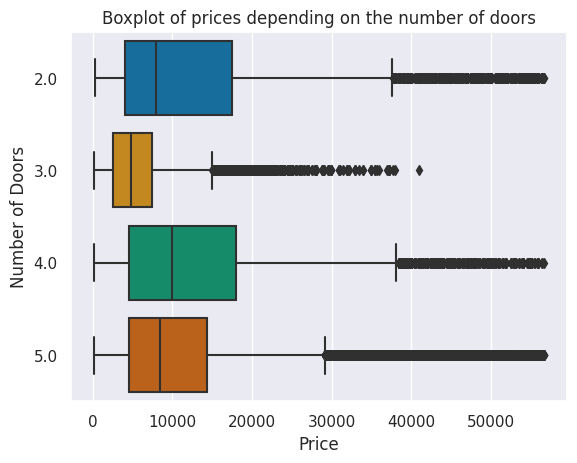
\includegraphics[width=\linewidth]{number of doors.png}
    \caption{Caption for Image 1}
    \label{fig:image1}
  \end{subfigure}
  \hfill
  \begin{subfigure}{0.48\textwidth}
    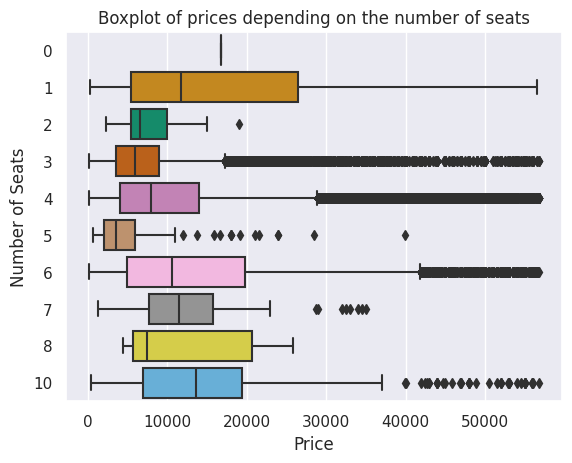
\includegraphics[width=\linewidth]{number of seats.png}
    \caption{Caption for Image 2}
    \label{fig:image2}
  \end{subfigure}
  \caption{Boxplots of prices depending on integer variables}
  \label{fig:twoimages}
\end{figure}
\FloatBarrier

\noindent Finally, we analyzed the qualitative data, also using boxplots. The graph on the left revealed (significant) differences in the dispersion of the data according to fuel type. The boxplots show marked variations between different fuel categories, highlighting the potential impact of this variable on vehicle price prediction. 
The middle boxplot, associated with vehicle types, showed a similar distribution for the first seven types, while the last two types "Car Derived Van" and "Limousine" stand out clearly from the others by tending towards lower prices, probably due to a reduced amount of data. 
Finally, the last boxplot on the right shows a trend whereby cars with automatic gearboxes tend to be more expensive than those with manual gearboxes.

\FloatBarrier
\begin{figure}[ht]
  \centering
  \begin{subfigure}{0.36\textwidth}
    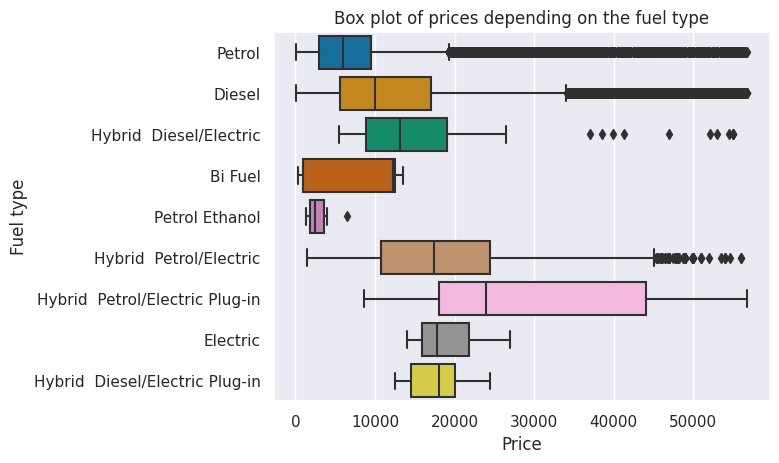
\includegraphics[width=\linewidth]{fuel type.png}
    \caption{Caption for Image 1}
    \label{fig:image1}
  \end{subfigure}
  \hfill
  \begin{subfigure}{0.32\textwidth}
    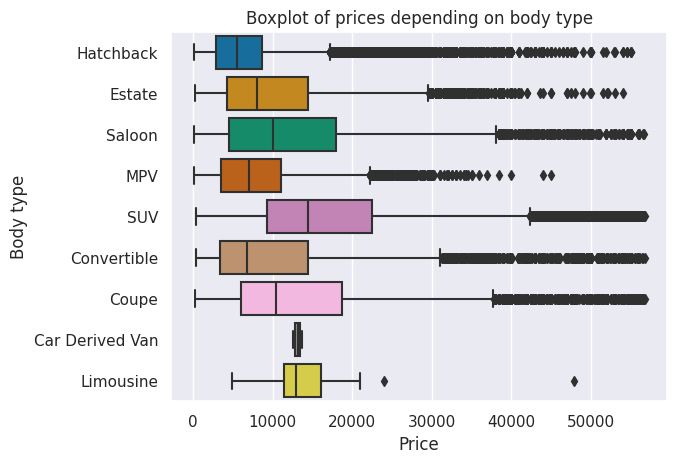
\includegraphics[width=\linewidth]{body type.png}
    \caption{Caption for Image 2}
    \label{fig:image2}
  \end{subfigure}
  \hfill
  \begin{subfigure}{0.30\textwidth}
    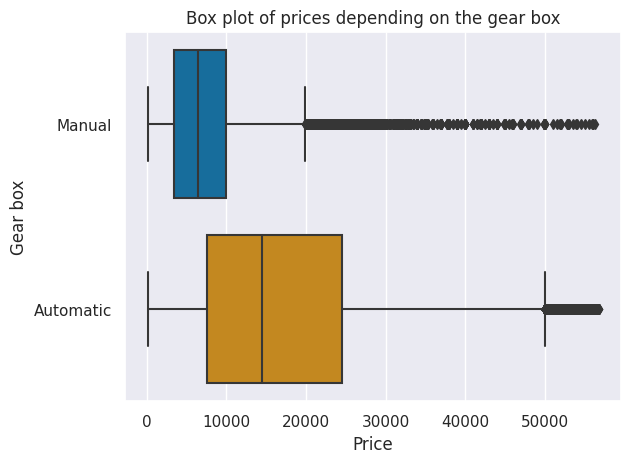
\includegraphics[width=\linewidth]{gear box.png}
    \caption{Caption for Image 3}
    \label{fig:image3}
  \end{subfigure}
  \caption{Dependance between qualitative variables and the price}
  \label{fig:threeimages}
\end{figure}
\FloatBarrier



\paragraph{Data Prepossessing}
~~\\

\noindent In order to carry out preprecessing in a uniform and structured way, we have opted to use object-oriented programming (OOP). This is a method of creating classes to create and manipulate objects, in this case observations. This class, called preprocess Ad Table Trim, enabled efficient and optimized preprocessing (to be seen). First, we renamed the columns of the merged table to have standardized column names so as to have the same structure for all variables. Then, after an analysis of the missing values, we decided to delete them, considering our already very large and complete database. For some variables, such as "average mpg", "engine size", "engine power" and "top speed", we decided to impute the missing values by the specific average for each type of model. We made this choice because there were many missing values in these variables, which we felt were very important in our database. \\

\noindent Next, we converted all categorical data into numerical format using the "one hot encoding" function, which creates binary variables, making it easier to integrate this information into machine learning models. After identifying outliers (show some calculations or graphs), we removed the 1\% highest prices and data with zscores greater than 4. Scoring is a calculation (put calculation) that assigns a score to values that appear to be outliers. This step led to the removal of around 10K observations, representing x\% of our initial database. (see for the number of NaNs deleted).\\

\noindent Finally, the last step was the standardization (calculation) of the values, an essential step in machine learning. It allows us to have data on a common scale, making them comparable. \\

\noindent Thanks to the creation of this automated class, we obtain a class that ensures the creation of a coherent data set, ready to be exploited for training machine learning models. \\


\subsubsection{Image data}
\paragraph{Data Description}
~~\\
\noindent Le fichier ZIP contient 1 451 784 images de voiture. Elles ont déjà été retravaillé par les créateurs de la base de données. Les backgrounds sont tous blanc, les images sont bien recentrées, et surtout, la position de la voiture a été prédite. Cette prédiction est disponible dans la table Images. C’est une information importante, car nous commencerons par essayer de prédire les prix des voitures qui ont été prise de face.

\noindent Nous avions pour projet de concaténer le modèle CNN aux données numériques. Cependant, nous avons passé beaucoup de temps à essayer de preprocess les images en créant les liens via \textit{Ad} et \textit{Trim}. Pour des raisons techniques, cette méthode n'a pas abouti et c'est pourquoi nous avons ensuite décidé d'utiliser seulement \textit{Price}. Cette table contient un prix par modèle de voiture et par année. En la liant à la table \textit{Image}, nous avons pu obtenir un nombre assez conséquent d'image labellisé par des prix, pour réentrainer un modèle CNN.



\paragraph{Price distribution}
~~\\
\noindent Etant donné que les prix et modèles que nous avons preprocess ne sont pas exactement les mêmes que pour la partie précédente, nous avons du ré-établir un choix de suppression des outliers. Comme nous pouvons le voir ci-dessous, Nous avons beaucoup d'outliers au delà de 80k euros. Pour garder un nombre conséquent d'images et pour complexifier la taxe à notre modèle CNN, nous avons décider de ne pas garder les images ayant un prix associé supérieur à 85k euros.

\begin{figure}[ht] 
    \centering

    \begin{subfigure}[b]{0.45\textwidth} 
        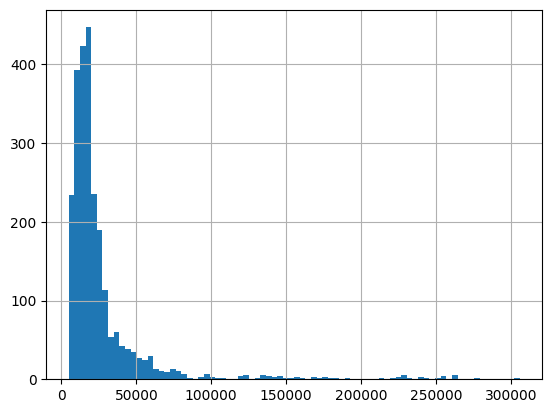
\includegraphics[width=\textwidth]{price_image_distribution_1.png}
        \caption{All images}
        \label{fig:image1}
    \end{subfigure}
    \hfill % Ajoute un espace entre les deux images
    \begin{subfigure}[b]{0.45\textwidth}
        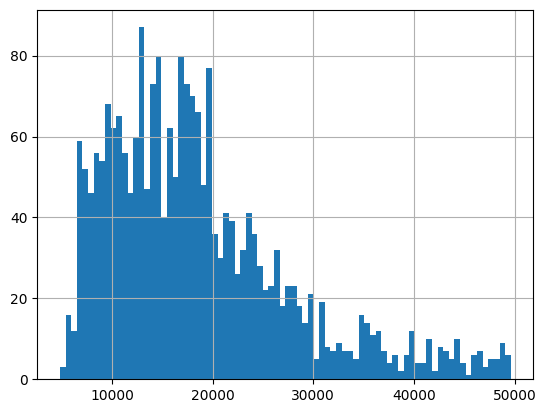
\includegraphics[width=\textwidth]{price_image_distribution_2.png}
        \caption{Without outliers}
        \label{fig:image2}
    \end{subfigure}

    \caption{Distribution of prices for front view images}
    \label{fig:Price distribution}
\end{figure}


\newpage
\paragraph{Data Prepossessing}
~~\\
\noindent Le data preprocessing de ces données s'est trouvé être très technique. Comme pour le premier preprocessing, nous avons créé une classe dans le fichier \textit{library.py} ayant pour nom \textit{DVMdataset}. 

\noindent Avant tout, les tables \textit{Image} et \textit{Price} sont concaténé de manière à ce que chaque donnée dans \textit{Image} ait un prix. C'est le dataframe des deux tables concaténé qui sera l'input de la classe. \noindent Notre classe comporte trois méthodes. 

\begin{itemize}
    \item \textit{unpack all images} : itère chaque donnée de notre dataframe et va trouver en navigant dans les folders du fichier ZIP l'image associée. Une fois que cette image est trouvée (si elle l'est), le prix de la donnée lui est attribuée. 

    \item \textit{getitem} : returns an image with a certain transformation strategy, and with its index. It is a necessary element to use pytorch dataloaders, and it also allowed us to print our images in an easy way.
    
    \item \textit{len} : returns the number of images in our dataset.
\end{itemize}


\noindent Explain the path of images



\subsection{Machine Learning Algorithms}
\subsubsection{Methods for Categorical and Numerical Data}
Short presentation / advantages and disadvantages / Reason of choice:
\begin{itemize}
    \item XGB
    \item Random Forest?

    \item KNN?
    \item PCA 
    \item PDP, SHAPLEY?
\end{itemize}

\subsubsection{Multiple layers Neural Network}

\noindent Explain what is a neural network. Explain what are the dropout probabilities, the batch size, the learning rate, the activation functions etc...

\paragraph{Tuning the neural network}

\noindent To tune our hyper parameters, we have decided to focus on five parameters and swap them using the library \textit{Weights and Biases} (also known as \textit{Wandb}) : the \textit{dropout probabilities}, the \textit{activation function}, the \textit{batch size}, the \textit{learning rate} and the \textit{number of epoch}. In fact, the best number of epochs has been re-selected while training our best model during the cross validation.

\noindent For some hyper parameters, we set them up with a minimum and maximum value. During the run, \textit{Wandb} swap these parameters by taking a random number between bounds, following a certain distribution function. For other parameters, we chosen to set up some set of values. In this configuration, \textit{Wandb} does not draw a random value between two bounds, but a random value between different limited choices.


\begin{table}[h]
    \centering
    \caption{Parameters swapped through a distribution function}
    \label{table:Parameters swapped through a distribution function}
    \begin{tabular}{lrrrrrrr}
    \toprule
           & Minimum & Maximum & Distribution \\
    \midrule
     Learning rate & 0.0005 & 0.07 & Uniform  \\
     Batch size & 30 & 200 & Q\_log\_Uniform  \\
     Epoch & 3 & 15 & Q\_log\_Uniform  \\
    \bottomrule
    \end{tabular}
\end{table}

\begin{table}[h]
    \centering
    \caption{Parameters swapped with limited sets}
    \label{table:Parameters swapped with limited sets}

    \begin{tabular}{lrrrrrrr}
    \toprule
           & Set of possible values \\
    \midrule
     Activation function & \begin{tabular}[c]{@{}l@{}}Tanh\\ Sigmoid\\ Relu\end{tabular} \\
     Batch size & \begin{tabular}[c]{@{}l@{}}0.1, 0.1, 0.1, 0.1\\
                                 0.3, 0.2, 0.1, 0.1\\
                                 0.1, 0.1, 0.2, 0.3\\
                                 0.1, 0.4, 0.4, 0.1\\
                                 0.3, 0.1, 0.1, 0.3\end{tabular} \\
    \bottomrule
    \end{tabular}
\end{table}

\noindent The Table~\ref{table:Parameters swapped through a distribution function} presents the parameters we chosen to swap each parameters and the Table~\ref{table:Parameters swapped with limited sets} the parameters with fixed sets of possible values. 
To avoid over fitting, the maximum learning rate was set at 0.07 and to reduce the time of computation, the maximum number of epochs is set to 15. Since we are doing a regression and trying to predict prices, the rectified linear (\textit{Relu}) activation function should be the best activation function as it predicts only positive values. Meanwhile \textit{Sigmoid} is more appropriated for classification tasks and the hyperbolic tangent (\textit{Tanh}) only for ranges between -1 and 1. However, we wanted to check if the \textit{ReLu} would actually perform better and included the three choices in the parameter swap configuration.
\noindent For the \textit{dropout probabilities} we tried to make a mixture of possible probabilities. This method is fixed for a certain number of hidden layers. It could be optimized with an ingenious function that could randomly draw probabilities between 0 and 0,4.



\FloatBarrier
\begin{figure}[ht]
    \centering
    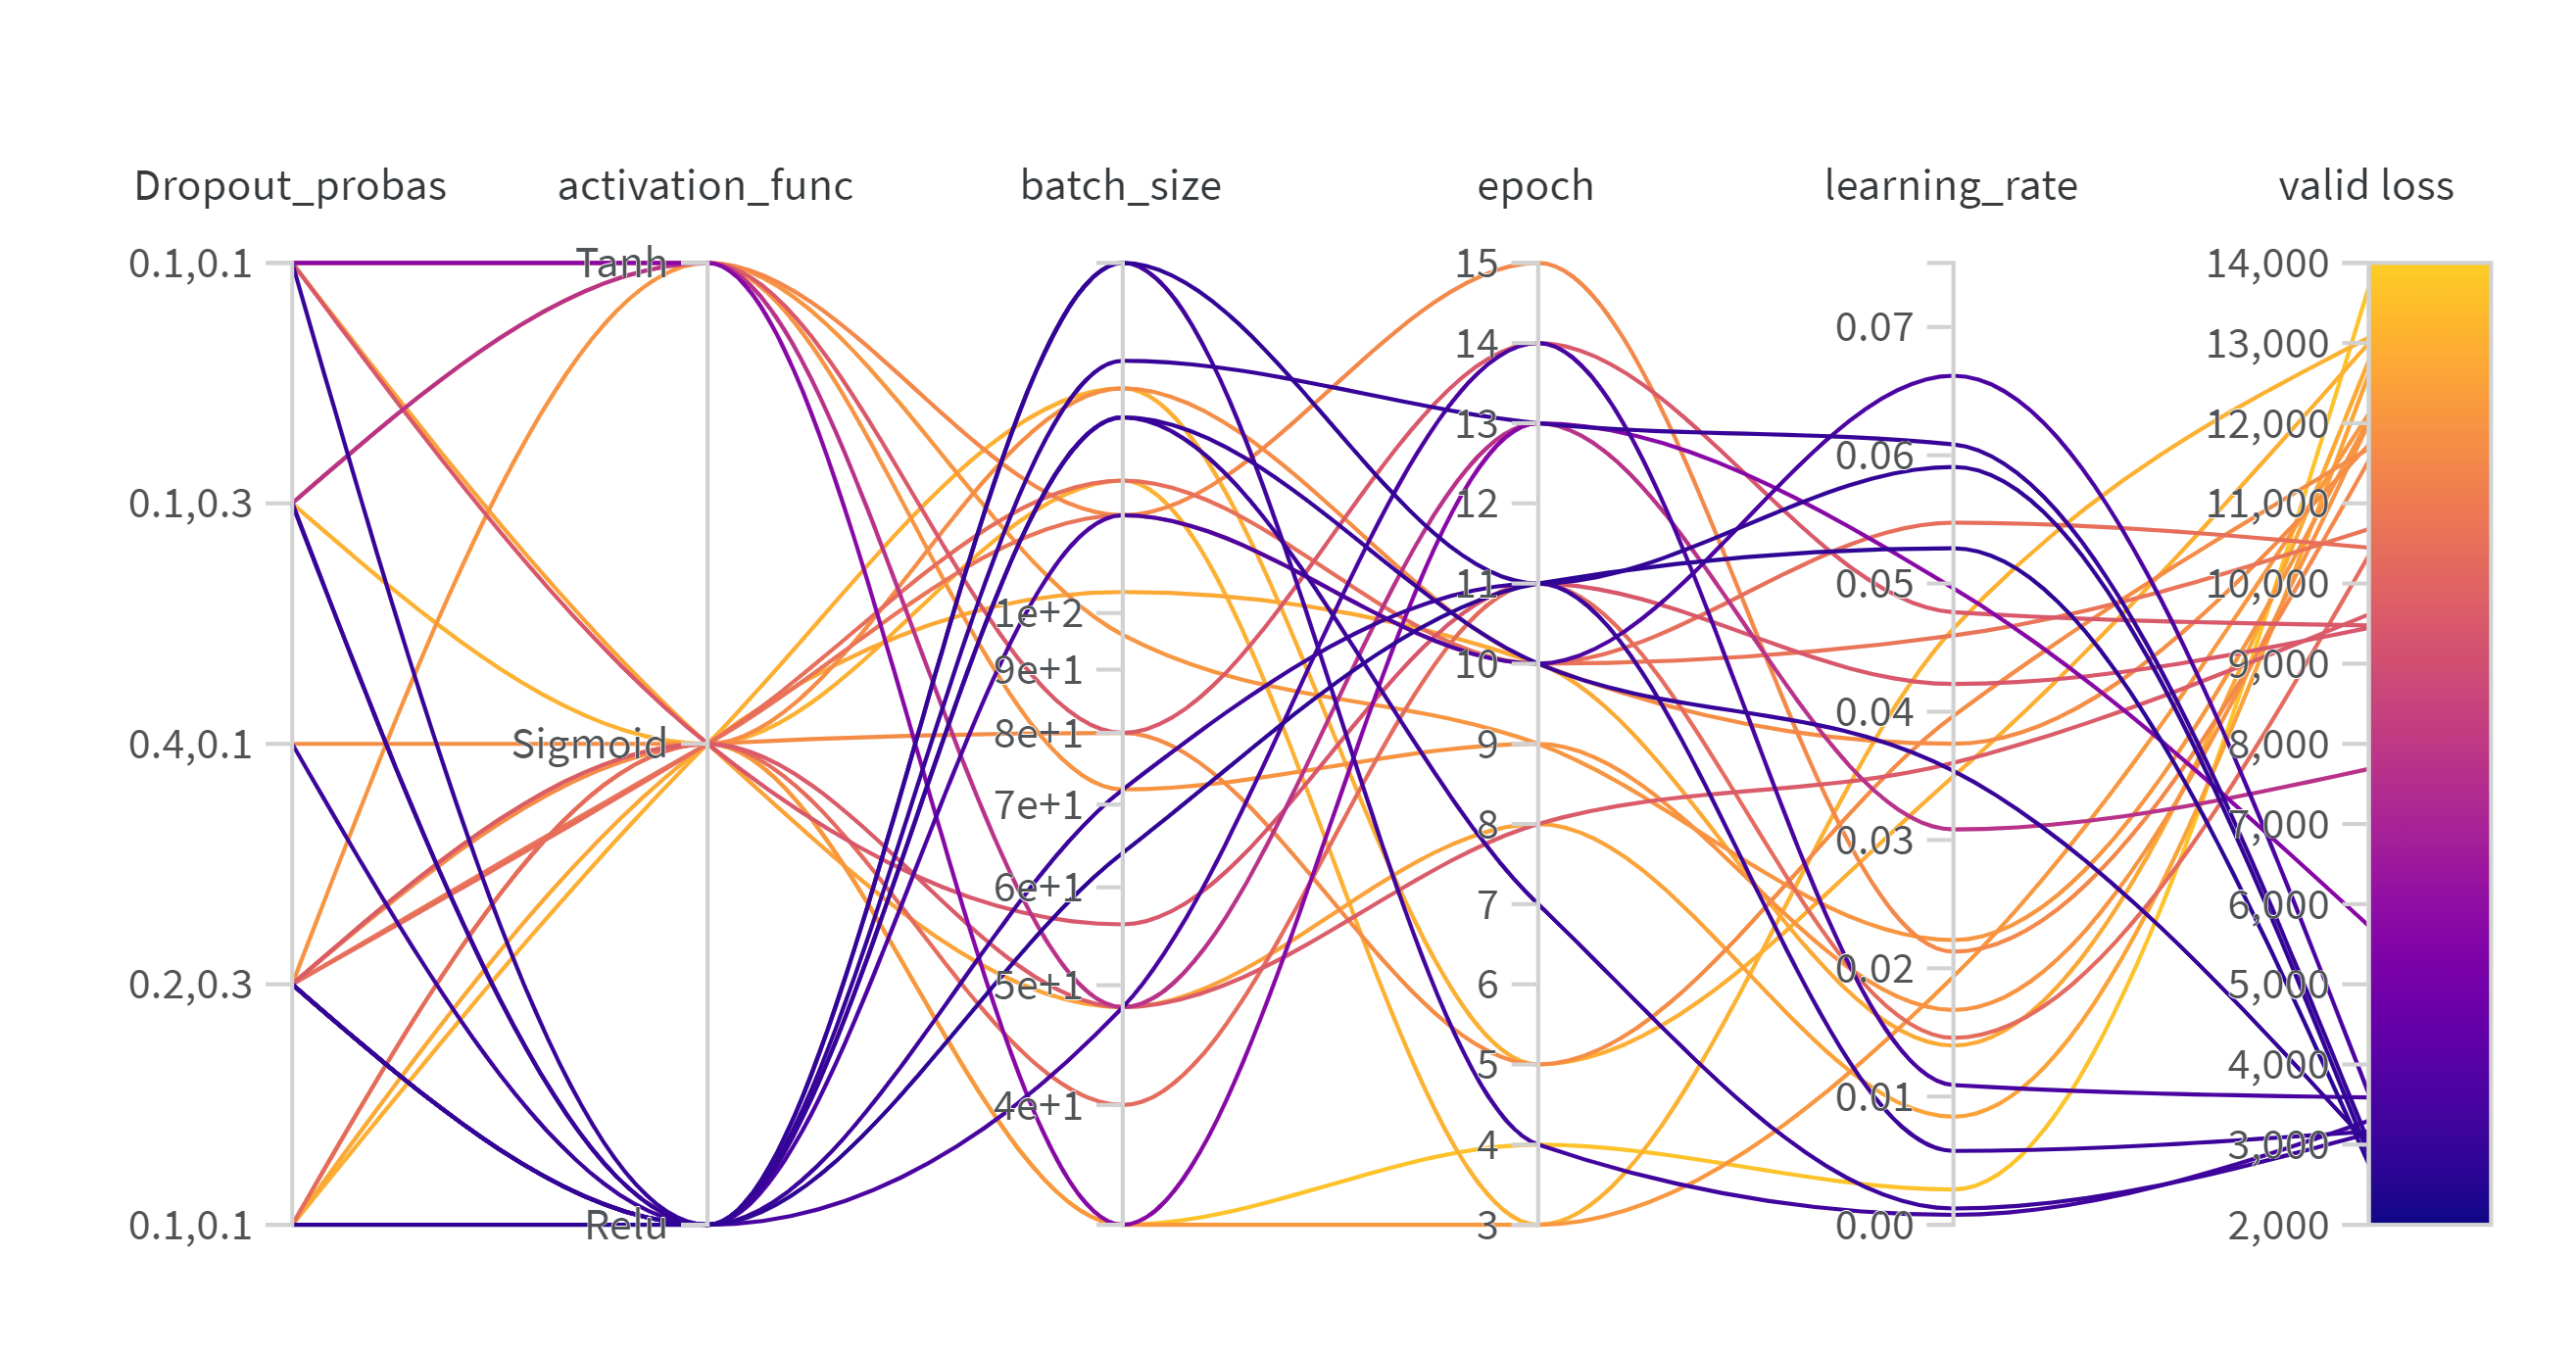
\includegraphics[width=1\textwidth]{wandbrun_1.png}
    \caption{Hyper parameters tuning results}
    \label{table:Hyper parameters tuning results MLP}
\end{figure}
\FloatBarrier

\noindent The Figure~\ref{table:Hyper parameters tuning results MLP} displays the result of \textit{Wandb} run. For thirty possible combinations of parameters drawn with our setting, we trained and evaluated the neural network with two different set of data (train and valid). Then, \textit{Wandb} shows the validation loss of each model with their respective parameter combinations. The path colour tends to a darker purple when the model had a low loss with the validation set, and to a clear yellow when it increases.
Thanks to this plot, it is straight to see that the models with a \textit{Relu} activation function tend to have pretty nice validation losses compared to the other functions.
We then decided to take the set of parameters with the lower validation loss to test our model with an other dataset. 

\subsubsection{Methods for image data}
Short presentation / advantages and disadvantages / Reason of choice:
\begin{itemize}
    \item CNN
    \item MLP
     \item PCA 
    \item PDP, SHAPLEY?
\end{itemize}

\subsubsection{Methods for mixed data}
\begin{itemize}
    \item Enter in hidden layers
    \item combine the data / models - but how?
\end{itemize}

\section{Results: Price estimation with classical data}
A detailed section: “Materials and Methods” presenting first the data used, the ways to collect and
format them; and a detailed description of the methods used in your analysis: theory elements on
the models used, empirical strategy (model selection, cross validation, grid search, etc.). Do not
forget to cite your sources.
Note: Your work should not be a catalogue of estimation methods. It is best to limit yourself to a
small number of methods, which you can present properly.

\subsection{Extreme Gradient Boosting Regression (XGBoost)}
\subsection{K-Nearest Neighbors (KNN)}
\subsection{Multilayer Perceptron (MLP)}

\section{Results: Price estimation with image data}
\subsection{Convolution Neural Networks (CNN)}



\section{Conclusion}
A conclusion recalling your major results and proposing possible future work and perspectives.


\end{document}
